%%%%%%%%%%%%%%%%%%%%%%%%%%%%%%%%%%%%%%%%%%%%%%%%%%%%%%%%%%%%%%%%%%%%%%%%%%%%%%%%
\chapter{ТЕСТИРОВАНИЕ, АНАЛИЗ ПОЛУЧЕННЫХ РЕЗУЛЬТАТОВ}
%%%%%%%%%%%%%%%%%%%%%%%%%%%%%%%%%%%%%%%%%%%%%%%%%%%%%%%%%%%%%%%%%%%%%%%%%%%%%%%%

\section{Тестовое окружение}

На сервере установлена операционная система Debian GNU/Linux 8.4 (jessie). На сервере установлен сервер IP-телефонии Asterisk 13.7.2. В конфигурационных файлах настроены звонки с номерами формата XXX, и добавлены внутренние номера, позволяющие звонить при помощи web-сокетов по порту 8088. Для этого создан DTLS-сертификат, и включена поддержка icesupport.\cite{asterisk} Также добавлены номера, позволяющие звонить при помощи обычных сокетов по порту 5060.

На этом же сервере установлена CRM-система SalesPlatform vtiger CRM 6.4, которая работает на сервере Apache 2.4.10, в связке с PHP 5.6.22-0+deb8u1 и MySQL Server 5.5.49-0+deb8u1. Файлы разрабатываемого модуля помещены в корень CRM-системы. Чтобы подключить JavaScript файл к данной CRM-системе, необходимо добавить в базу данных CRM-системы в таблицу vtiger\_links запись c полями: linkurl - название файла (в нашем случае softPhone.js), linktype - HEADERSCRIPT, tabid - 0.\cite{vtiger_db} В этом случае скрипт будет выполнятся при каждой загрузке страницы.

Тестирование проводилось на браузерах Iceweasel 38.7.1, Mozilla Firefox 47.0, в них звонок работает хорошо. Также проводилось тестирование в браузерах Google Chrome 50.0.2661.75, Opera 38.0.2220.31, но на них не удалось полностью управлять звонком: иногда голос передавался только в одну сторону, иногда не удавалось его завершить. Однако следует заметить, что демо-версия sipML5 клиента\cite{sipML5_demo} работает на данной тестовой системе так же. В связи с этим можно сделать вывод, Google Chrome ведёт себя так из-за нововведения в версии 47, которое запрещает функцию getUserMedia() если используется протокол http, и позволяет её только для https.\cite{chrome_https}

\section{Функциональное тестирование}

Требования к работе модуля:
\begin{itemize}
\item Аутентификация и деаутентификация на сервере.
\item Сессия аутентификации должна корректно переходить из одного состояния в другое.
\item Корректные инициализация вызова и воспроизведение рингтона и гудков.
\item Сессия звонка должна корректно переходить из одного состояния в другое.
\item При звонке передача голоса должна быть в обе стороны.
\item В графическом интерфейсе в определённые состояния звонка должны быть неактивны определённые кнопки. Например, в момент разговора кнопка звонка должна быть выключена и доступна только кнопка сброса.
\item Корректная обработка звонков на несуществующие номера.
\end{itemize}

Функциональное тестирование проводилось вручную. Проверялись инициализация вызова как входящего, так и исходящего. Проверялось завершение вызова, инициируемое как нашим клиентом, так и клиентом собеседника. Завершение вызова проверялось как в момент разговора, так и в момент до снятия трубки.

На рисунках \ref{image:test1} - \ref{image:test8} изображён корректный графический интерфейс модуля в разных состояниях.

\begin{figure}[h!]
\center{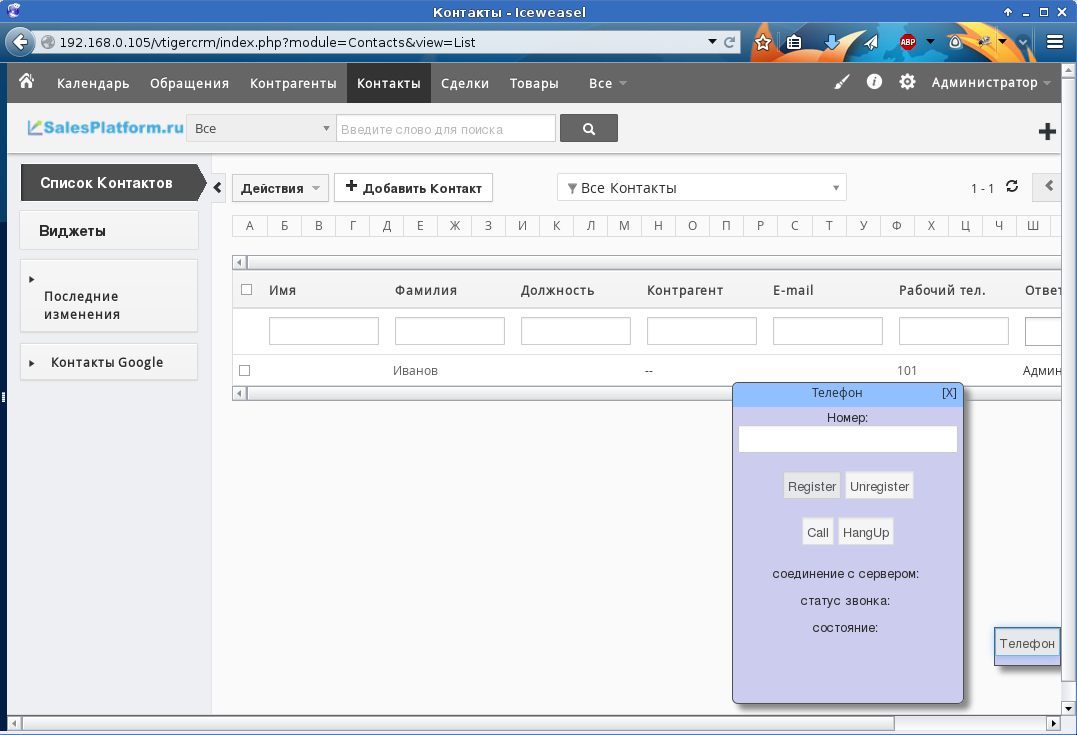
\includegraphics[width=0.75\linewidth]{test1}}
\caption{Модуль в CRM-системе SalesPlatform vtiger CRM 6.4, начальное состояние модуля}
\label{image:test1}
\end{figure}

На рисунке \ref{image:test1} видно кнопку "телефон". Это скользящая кнопка, выполняет функцию скрытия и отображения плавающего окна софт-фона.

\begin{figure}[h]
\center{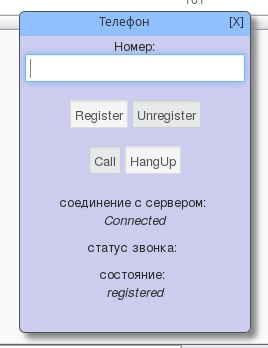
\includegraphics[width=0.4\linewidth]{test2}}
\caption{Состояние после аутентификации на сервере}
\label{image:test2}
\end{figure}

\begin{figure}[h]
\center{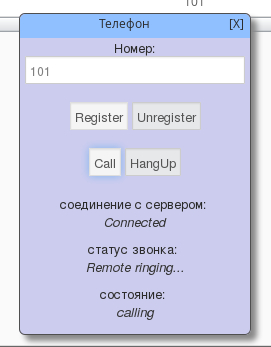
\includegraphics[width=0.4\linewidth]{test3}}
\caption{Состояние исходящего звонка (воспроизводятся гудки)}
\label{image:test3}
\end{figure}

\begin{figure}[h]
\center{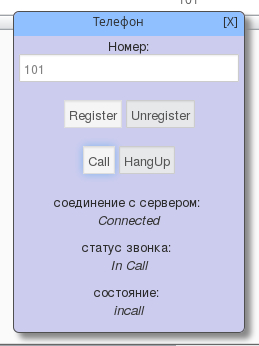
\includegraphics[width=0.4\linewidth]{test4}}
\caption{Состояние в процессе звонка}
\label{image:test4}
\end{figure}

\begin{figure}[h]
\center{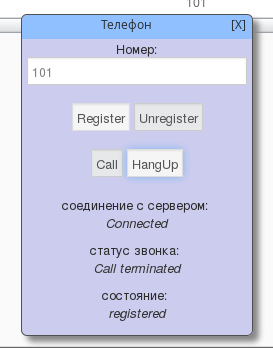
\includegraphics[width=0.4\linewidth]{test5}}
\caption{Состояние завершения звонка, такое же как и состояние после аутентификации на сервере}
\label{image:test5}
\end{figure}

\begin{figure}[h]
\center{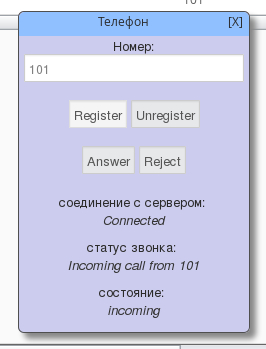
\includegraphics[width=0.4\linewidth]{test6}}
\caption{Состояние входящего звонка (воспроизводится рингтон)}
\label{image:test6}
\end{figure}

\begin{figure}[h]
\center{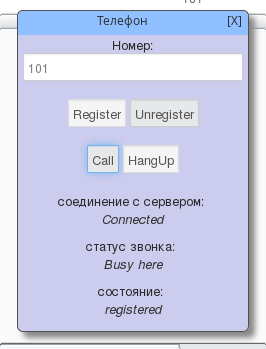
\includegraphics[width=0.4\linewidth]{test7}}
\caption{Вызываемый абонент занят}
\label{image:test7}
\end{figure}

\begin{figure}[h]
\center{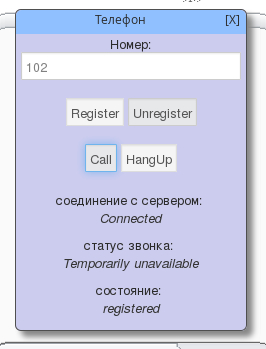
\includegraphics[width=0.4\linewidth]{test8}}
\caption{Вызываемый абонент недоступен}
\label{image:test8}
\end{figure}

Тестирование проводилось по ходу разработки, помогало выявить следующие функциональные ошибки: некорректное состояние сессии звонка, односторонняя передача голоса и некорректное состояние графического интерфейса.
